\documentclass[letterpaper,twocolumn,showkeys, 12pt]{article}
\usepackage[utf8]{inputenc}
\usepackage[T1]{fontenc}
\usepackage[margin=20mm]{geometry}
\usepackage[french]{babel}
\usepackage{graphicx}
\usepackage{lipsum}
\DeclareGraphicsExtensions{.pdf}

\title{Étude du réseau de collaboration des étudiants en écologie }
\author{Étienne Lacroix-Carignant\(^1\), Thomas Martel\(^1\), Vincent Moreau\(^1\), \\ Louis Plante\(^1\), Samuel Provencher-Tardif\(^1\) \\
\\ \(^1\) Baccalauréat en Écologie, Université de Sherbrooke}
\date{24 Avril 2020}

\begin{document}

\maketitle

\begin{abstract}
    L'analyse de réseaux permet de dégager des tendances à partir d'une grande quantité de données inter-reliées et est de plus en plus populaire maintenant que les outils informatiques sont assez puissants pour les réaliser. Nous aurons recours à cette technique pour étudier les relations de collaboration entre les étudiants au baccalauréat à l'Université de Sherbrooke qui ont suivi le cours BIO500 à la session d'hiver 2020. La réalisation du code et des figures ainsi que le traitement des bases de données suivent les principes de bases de la science reproductible et ont été montés de façon à être entièrement réplicables.
\end{abstract}

\section*{Introduction}
\noindent Les réseaux sont des outils de représentation très utiles en écologie pour représenter les interactions entre plusieurs niveaux d’organisation. Dans le règne animal, un type de réseau fréquent est la représentation du réseau trophique. Ce type de réseau permet d’avoir une idée, entre autres, sur l’identité des espèces clés et des « top prédateurs ». Ces informations sont très importantes dans le domaine de la conservation par exemple. En effet, il est important de connaître les interactions entre un prédateur qu’on veut contrôler et le reste des organismes présents pour pouvoir émettre des hypothèses juste sur l’impact potentiel d’un tel contrôle. Il est même possible d’établir ces interactions prédateurs-proies pour des espèces éteintes depuis longtemps (e.g \cite{chevrinais_early_2017}). Cependant, ce type de relation n’est pas vraiment applicable aux êtres humains. Cela ne veut pas dire pour autant que les réseaux ne sont peuvent pas représenter des interactions pertinentes chez cette espèces. Un type de relation intéressante à analyser chez les humains, plus particulièrement chez les scientifiques est le réseau de collaboration entre les scientifiques. L’analyse de ces collaborations sont de plus en plus d’actualité avec la crise de reproductibilité que subit présentement le milieu des sciences et l’ouverture des sciences pour contrer cette crise. Ces collaborations s’établissent tôt dans le parcours d’un scientifique. Dans le cadre de notre cours, nous avons établis un tel réseau de collaboration entre les étudiants en biologie de l’Université de Sherbrooke. Nous avons aussi analysé ce réseau pour en ressortir certaines propriétés qui nous permettent de mieux comprendre la nature, la diversité et la force de ces collaboration. Dans le cadre de ce travail, nous nous sommes intéressé à voir si les différences de connectivité entre les étudiants sont imputables à une différence dans le programme d'étude ou à une différence dans l'année de début du baccalauréat. 


\section*{Méthodologie}

\begin{table*}[h]
\centering
\caption{Statistiques d'intérêt du réseau}
\label{my-label}
\begin{tabular}{c c c}
Statistique & Nom(s) & Nombre   \\
\hline
Nombre de noeuds & & 185\\
Nombre de collaborations uniques & & 2243\\
Plus grand nombre de collaborations uniques & Camille Rondeau-St-jean & 34  \\
Plus grande affinité entre deux étudiants & Joelle Spooner et Charlotte Tessier-Larivière & 16  \\
\hline
\end{tabular}
\end{table*}

Au cours des derniers mois, les étudiants du cours BIO500 ont été appelé à réaliser une étude du réseau de collaborations entre les étudiants en biologie. Pour ce faire, les étudiants ont dû énumérer toutes les collaborations réalisées dans le cadre de travaux d’équipes au cours de leur parcours à l’Université de Sherbrooke. 

Dans une première table, nous avons placer plusieurs variables relatives aux étudiants inclus dans le réseau. Les noms des étudiants sont inscrits de manière standardisée afin de simplifier la mise en commun des tables provenant des autres équipes. Ici, l'identifiant d'un étudiant correspond à son nom de famille, suivi de son prénom, séparés d'un trait souligné. Ces identifiants ne contiennent ni caractères avec accent, ni majuscules, ni trait d'union. La session de début du baccalauréat est notée avec la première lettre de la saison (A pour automne ou H pour Hiver) de la session. Le programme d’étude en biologie était inscrit sans accent.Les étudiants qui n’étudiait pas ou plus en biologie à l'hiver 2020, on inscrit « autre ». La participation au régime de stage coopératif est inscrite en binaire où 1  pour oui et 0 pour non. On réfère à cette table avec l'appellation \textit{table étudiants}. Dans une seconde table, nous avons recensé les collaborations pour chaque travaux réalisé par les étudiants inclus dans le réseau. Les noms des deux étudiants ayant collaboré était inscrit selon le standard établi. Le sigle du cours dans lequel les élèves ont collaboré était inscrivent en majuscule et sans espace. L’année de collaboration était également inscrite.On réfère à cette table avec l'appellation \textit{table collaborations}. Dans une troisième table, nous avons placé l'information relative aux cours donnant lieu aux collaborations. On y trouve une colonne par variable d'intérêt, soit le sigle du cours, le nombre de crédits lui étant rattacher, le type de cours, obligatoire ou optionnel et le type de travail. Lorsqu'un cours donnait lieu à plusieurs travaux, le travail pris en compte était choisi selon l’ordre de priorité suivant : oral , ecrit, labo et finalement terrain. On réfère à cette table avec l'appellation \textit{table cours}.

Ces fichiers sont importé dans le logiciel d’analyse statistique R (version 3.6.3) en format CSV. Des erreurs ont été fait lors de la saisie des données (doublons, syntaxes, orthographes, etc). Pour corriger ces erreurs, nous avons développé des boucles, avec une connaissance \textit{a priori} des erreurs présentes. La base de données est gérée à l’aide du système de gestion de données SQLite3 qui est implémenté dans R avec le package (package RSQLite version 2.2.0). L’attribut étudiant est la clé primaire de la \textit{table etudiants}. Dans la \textit{table collaborations}, tous les attributs sont des clés primaires, les attribut  etudiant1  et  etudiant2  sont des clés étrangères faisant référence à l’attribut  nomprenom  de la table  etudiants  et l’attribut « sigle » est une clé étrangère faisant référence à l’attribut « sigle » de la table  cours. Dans la table « cours », l’attribut  sigle  est une clé primaire. 

\section*{Résultats}

Sur 185 étudiants ayant travaillé avec des étudiants du cours BIO500, plus de la moitié étudiaient au baccalauréat en écologie, avec une faible proportion en biologie moléculaire et en microbiologie. Le programme d'étude de plusieurs étudiants est inconnu; ces données sont regroupées dans la colonne "Autre" à la Figure 1. La majorité des collaborations ont lieu entre des étudiants en écologie; les collaborations avec des étudiants d'autres programme est marginale, comme on le voit sur la figure 2 et 3. La figure 4 permet de visualiser les liens entre les étudiants selon l'année du commencement de leur baccalauréat. Des groupes sont bien visibles, et abordés plus en détail dans la discussion. Des exemples de requêtes interrogeant la base de données qui a été compilée sont visibles dans la Table 1.


\begin{figure}[h]
    \centering
    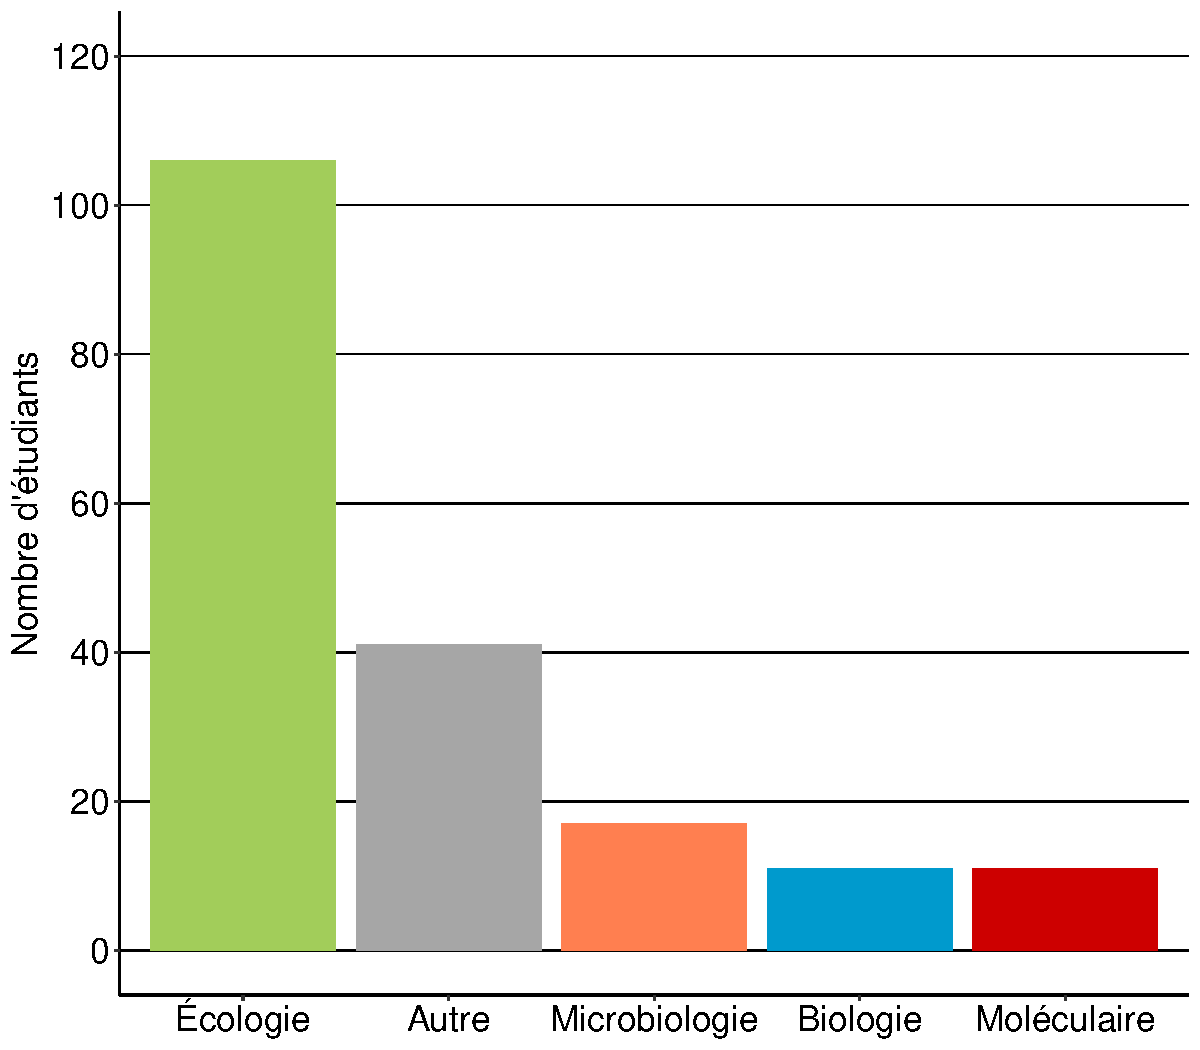
\includegraphics[width=0.5\textwidth]{Figure 1.pdf}
    \caption{Répartition des 185 étudiants répertoriés lors de cette étude dans les 4 concentrations en Biologie ou autres programmes à l'UdeS.}
    \label{fig:barplot1}
\end{figure}



\begin{figure}[h]
    \centering
    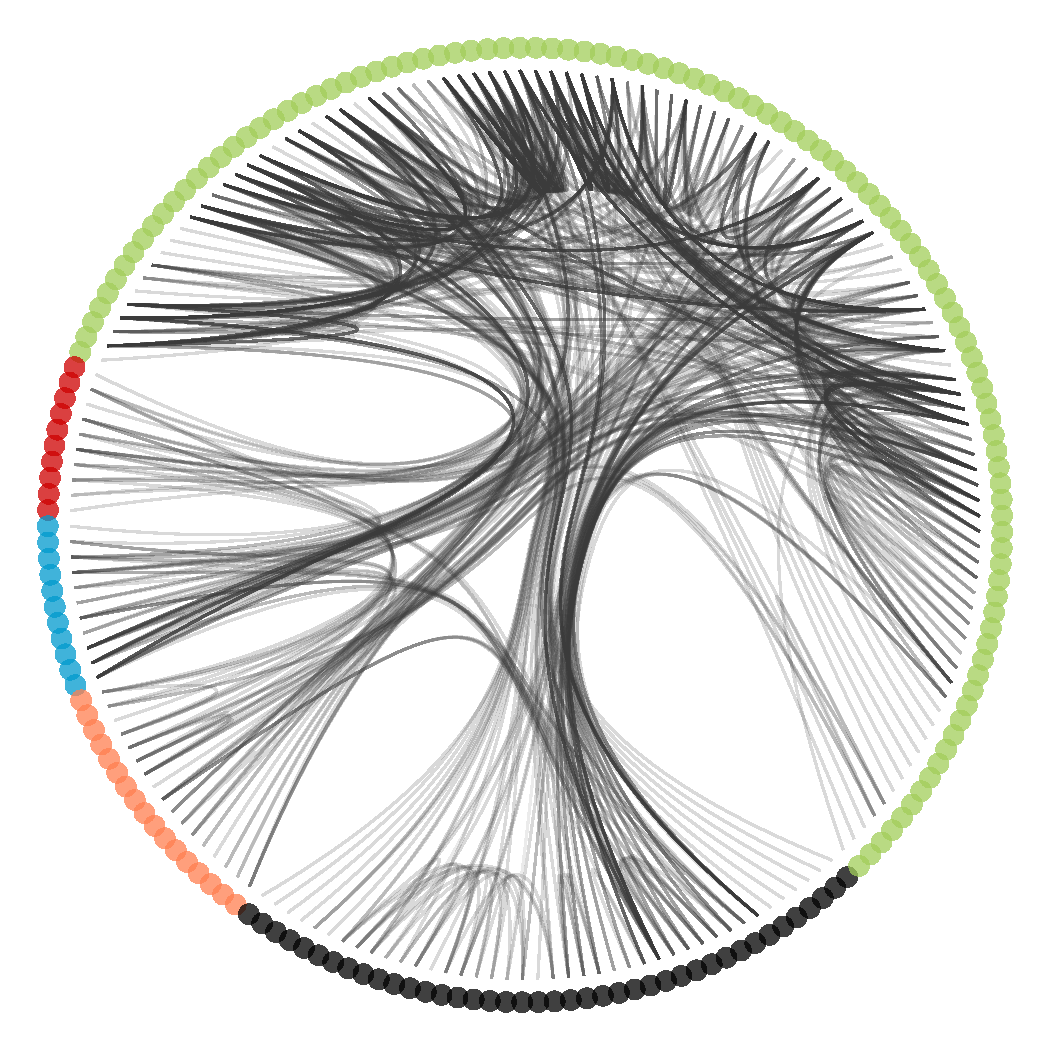
\includegraphics[width=0.5\textwidth]{Figure 2.pdf}
    \caption{Représentation hiérarchique du réseau d'interactions des étudiants en biologie de plusieurs concentrations différentes: Écologie (vert), Microbiologie (Orange), Biologie générale (Bleu), Biologie moléculaire (Rouge) et autres programmes (Noir).}
    \label{fig:barplot1}
\end{figure}


\begin{figure*}[h]
    \centering
    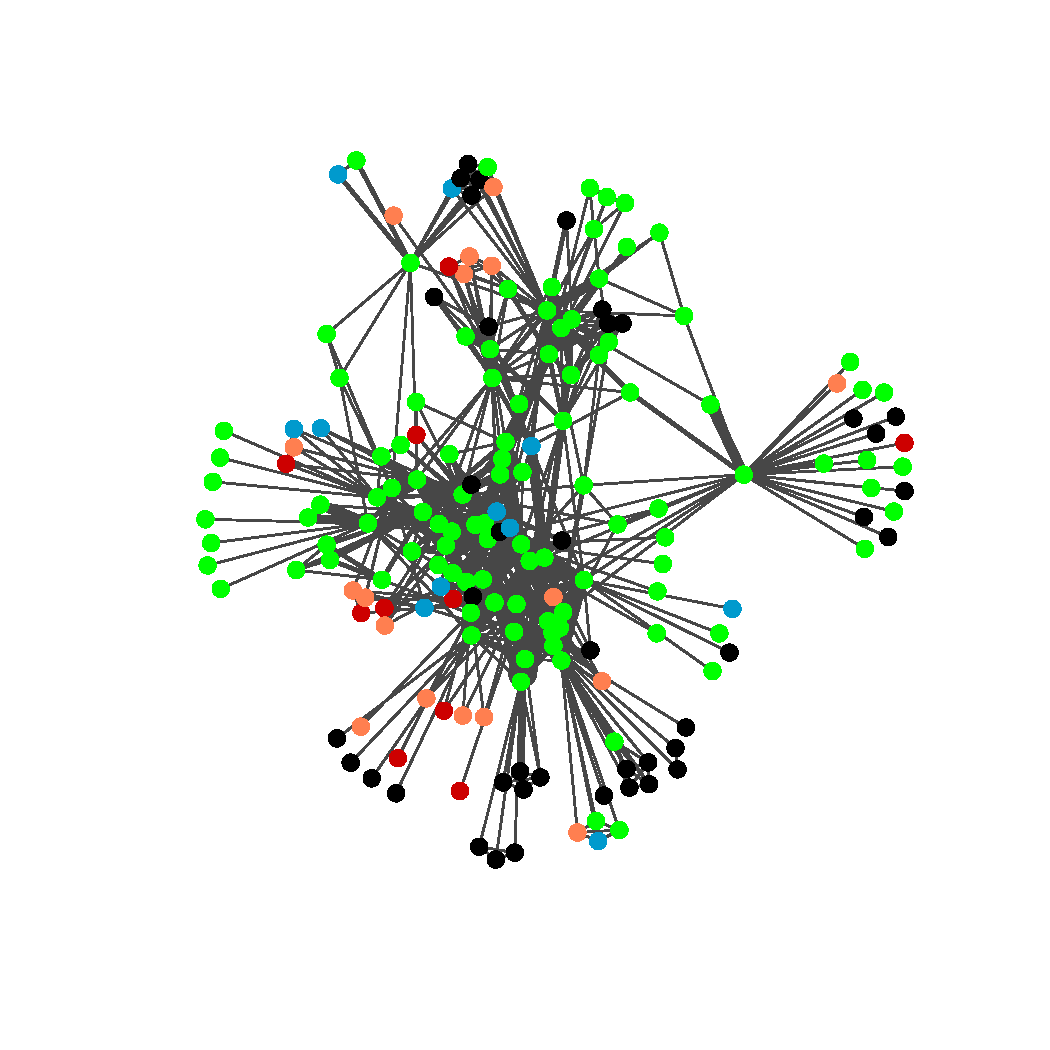
\includegraphics[width=400,trim={20mm 20mm 20mm 20mm},clip]{Figure 4.pdf}
    \caption{Représentation du réseau d'interactions des étudiants en biologie de plusieurs concentrations différentes: Écologie (vert), Microbiologie (Orange), Biologie générale (Bleu), Biologie moléculaire (Rouge) et autres programmes (Noir). La position des noeuds est déterminée selon l'algorithme de Fruchterman.}
    \label{fig:barplot1}
\end{figure*}

\begin{figure*}[h]
 \center
  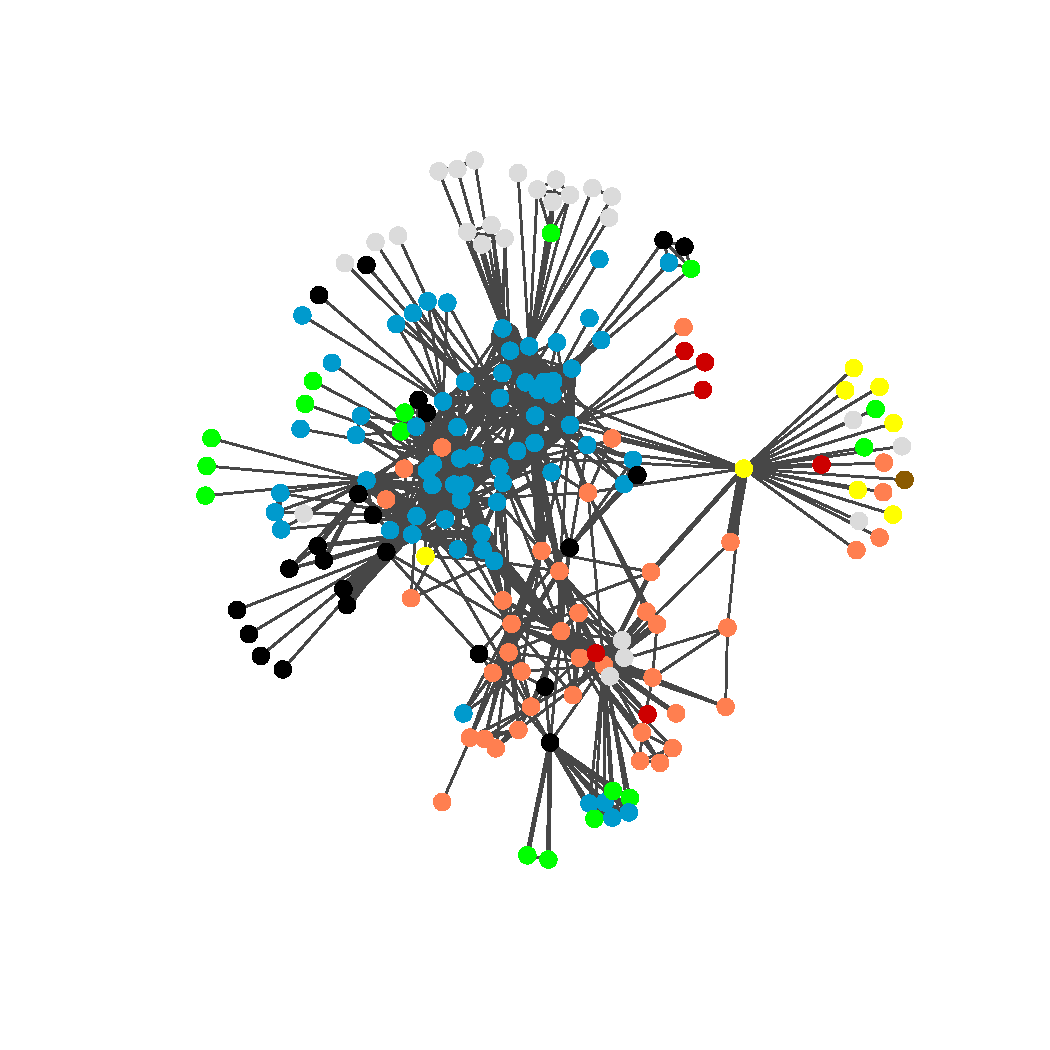
\includegraphics[width=400,trim={20mm 20mm 20mm 20mm},clip]{Figure 3.pdf}
  \caption{Représentation du réseau d'interactions des étudiants en biologie selon l'année de commencement du Baccalauréat: 2019 (Noir), 2018 (bleu), 2017 (vert), 2016 (orange), 2015 (rouge), 2014 (jaune), 2012 (orange-brun) et NA (gris pale). La position des noeuds est déterminée selon l'algorithme de Fruchterman.}
  \label{Figure 3}
\end{figure*}


\section*{Discussion}

Comme il fallait s'y attendre pour un cours obligatoire dans le baccalauréat en écologie, la majorité des étudiants de BIO500 appartiennent à ce programme (Figure 1 et 2), et la vaste majorité des collaborations répertoriées ont eu lieu entre des étudiants de ce programme (Figure 2 et 3). Cette dernière figure n'est donc pas particulièrement instructive, mais on constate toutefois que les étudiants appartenant à d'autres programmes apparaissent surtout en périphérie de la figure et ont moins de liens en général que les gens en écologie. Cela se fait aussi ressentir dans le nombre de collaborations entre chaque paire d'étudiant, les traits plus épais sur la figures étant surtout rencontrés dans le centre du graphique entre des gens du même programme. Il est logique que des étudiants du même programme aient davantage de possibilités de collaborations, puisqu'ils ont plus de chances d'avoir des cours en commun. Certains étudiants sont portés à travailler avec moins de personnes mais à leur être très fidèle alors que d'autres sont plus généralistes et ont un réseau de collaborations plus vaste et ont moins tendance à retravailler avec les mêmes personnes (Table 1 et Figures 3 et 4). C'est un comportement intéressant dont les causes pourraient être explorées plus en détail.  Dans la figure 3, on discerne deux grands groupes assez mal bien délimités, mais l'information sur le programme d'étude n'offre pas d'explication évidente sur cette disparité. En observant la figure 4, l'explication saute aux yeux: les étudiants de cohortes différentes ont moins tendance à collaborer dans des travaux d'équipe. L'année d'entrée dans le programme d'étude est donc la variable qui semble avoir le plus d'influence sur les réseaux de collaboration de chaque étudiant du cours.

Le réseau décrit ici comprend des liens plus ou moins fort en les étudiants. On voit, sur la Figure 2, que le nombre moyen de collaborations par étudiant est environ de 1. En revanche, on observe aussi des fortes affinités (Table 1 et Figure 3 et 4). Ceci nous laisse penser que le réseau comprend des étudiants généraliste et des étudiants très spécifiques dans leurs collaborations, soit des spécialiste. On peut faire un parallèle entre ce réseau et la communauté de bourdons en Amérique du Nord, qui comprend elle aussi des généraliste et des spécialistes \cite{jacobson_decline_2018}

La présence dans la figure d'un étudiant avec pas moins de 17 collaborations uniques s'explique par l'année de son entrée dans le programme d'étude. La majorité des étudiants avec lesquels cette personne a travaillé ont eu le temps de terminer leurs études avant même que la majorité des étudiants ne commencent leurs études universitaires. 
\\
\\
\\
\\
\\
\\
\bibliographystyle{plain-fr}
\bibliography{reference}
\end{document}